\documentclass[aspectratio=169,11pt]{beamer}

% Shared style (ib-tutorials.sty at the repo root).
\makeatletter\def\input@path{{./}{../}}\makeatother
\usepackage{ib-tutorials}

\usepackage[utf8]{inputenc}
\usepackage{amsmath,amssymb}
\usepackage{booktabs}
\usepackage{array}
\newcolumntype{L}[1]{>{\raggedright\arraybackslash}p{#1}}
\usepackage{graphicx}
\graphicspath{{../pictures/5-visit/}{pictures/5-visit/}}
\usepackage{xcolor}
\usepackage{listings}
\usepackage{tikz}
\usetikzlibrary{arrows.meta,positioning,shapes.geometric,fit,calc}
\usepackage{hyperref}

\newcommand{\sourcecredit}[1]{\vfill\begin{flushright}\tiny\textcolor{DarkGray}{#1}\end{flushright}}
\newcommand{\gui}[1]{\textsf{\textbf{#1}}}

\lstset{
  basicstyle=\ttfamily\scriptsize\color{BlackGray},
  keywordstyle=\color{NavyBlue}\bfseries,
  commentstyle=\color{DarkGray}\itshape,
  stringstyle=\color{OliveGreen},
  showstringspaces=false,
  columns=fullflexible,
  keepspaces=true,
  breaklines=true,
  breakindent=1em,
  frame=single,
  framerule=0.4pt,
  rulecolor=\color{LightGray},
  backgroundcolor=\color{LightGray!30},
  xleftmargin=0.25em,
  xrightmargin=0.25em
}
\lstdefinestyle{shell}{morecomment=[l]{\#}}
\lstdefinestyle{python}{morecomment=[l]{\#}}
\lstdefinestyle{tiny}{basicstyle=\ttfamily\tiny\color{BlackGray}}
\lstdefinestyle{pytiny}{morecomment=[l]{\#},basicstyle=\ttfamily\tiny\color{BlackGray}}
\lstdefinestyle{shtiny}{morecomment=[l]{\#},basicstyle=\ttfamily\tiny\color{BlackGray}}

\title[VisIt on the cluster]{VisIt on the cluster}
\subtitle{Where the data are: VisIt scripts in batch jobs on Puma, a desktop on a compute node, X11, and client--server; a parallel engine; resampling, averages and movies without downloading the run}
\author[Miller]{Laura A. Miller}
\institute[UArizona]{Department of Mathematics, University of Arizona}
\date{Using IB Software \textbullet\ Part V \textbullet\ Chapter 31}

\begin{document}

% 1
\begin{frame}[plain]
\maketutorialtitlepanel{%
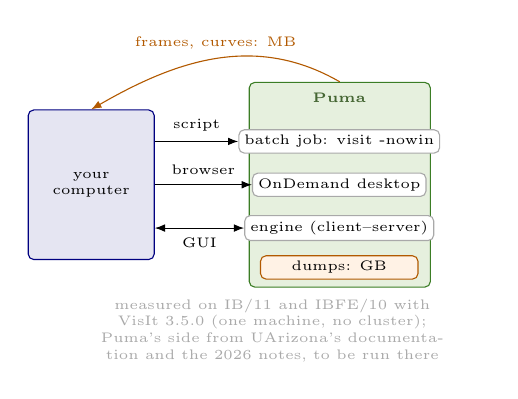
\begin{tikzpicture}[every node/.style={font=\tiny}, box/.style={draw, rounded corners=2pt, align=center, inner sep=2pt}]
  \node[box,draw=NavyBlue,fill=NavyBlue!10,minimum width=1.6cm,minimum height=1.9cm] (pc) at (0,0) {your\\computer};
  \node[box,draw=OliveGreen,fill=OliveGreen!10,minimum width=2.3cm,minimum height=2.6cm,anchor=west] (puma) at (2.0,0) {};
  \node[font=\tiny\bfseries,text=OliveGreen!70!black] at (3.15,1.1) {Puma};
  \node[box,draw=DarkGray,fill=white,minimum width=2.0cm] (job) at (3.15,0.55) {batch job: \code{visit -nowin}};
  \node[box,draw=DarkGray,fill=white,minimum width=2.0cm] (ood) at (3.15,0.0) {OnDemand desktop};
  \node[box,draw=DarkGray,fill=white,minimum width=2.0cm] (eng) at (3.15,-0.55) {engine (client--server)};
  \node[box,draw=orange!70!black,fill=orange!10,minimum width=2.0cm] (dumps) at (3.15,-1.05) {dumps: GB};
  \draw[-{Latex[length=1.3mm]}] (pc.east) ++(0,0.55) -- node[above,font=\tiny]{script} (job.west);
  \draw[-{Latex[length=1.3mm]}] (pc.east) -- node[above,font=\tiny]{browser} (ood.west);
  \draw[{Latex[length=1.3mm]}-{Latex[length=1.3mm]}] (pc.east) ++(0,-0.55) -- node[below,font=\tiny]{GUI} (eng.west);
  \draw[-{Latex[length=1.3mm]},orange!70!black] (puma.north) to[out=150,in=30] node[above,font=\tiny,text=orange!70!black]{frames, curves: MB} (pc.north);
  \node[text=DarkGray,align=center,text width=5.3cm] at (2.3,-1.85) {measured on IB/11 and IBFE/10 with VisIt 3.5.0 (one machine, no cluster); Puma's side from UArizona's documentation and the 2026 notes, to be run there};
\end{tikzpicture}}
\end{frame}

% 2
\begin{frame}{Learning goals}
\label{fr:goals}
\footnotesize By the end of this chapter you should be able to:
\begin{itemize}
  \item Say which of four ways to run VisIt with a cluster fits a task: a script in a batch job, a desktop on a compute node, X11 forwarding, or client--server.
  \item Get VisIt on Puma (the module, or your own install) and run a VisIt script there without a display.
  \item Turn a script tested on your computer into a batch job that writes frames, averages or resampled data next to the run, and check what it wrote.
  \item Start a parallel compute engine, and know when it helps.
  \item Use the 2020 cluster tutorial's recipes (IBFE meshes, resampling, VTK databases, averages over time) in VisIt 3.5.
\end{itemize}
\begin{punchbox}
\small Move the analysis to the data, not the data to the analysis: a 3D run's dumps are gigabytes, its frames and curves are megabytes.
\end{punchbox}
\end{frame}

% 3
\begin{frame}{Where this chapter comes from}
\label{fr:sources}
\scriptsize
\begin{itemize}
  \item \al{G. Hobson, ``Post-Processing IBAMR Simulation Data in VisIt on a Computing Cluster''} (Scripps Institution of Oceanography, UC San Diego, 23 September 2020; ``A contribution to the IBAMR Tutorials Research Group'', 32 slides): VisIt 3.1.2 installed from the tarball on UNC's Dogwood and Longleaf clusters, scripts recorded in the GUI and run with \code{visit -cli -nowin -s}, the rubber band, IBFE meshes, 3D resampling, VTK databases, averages over time, restarting a job.
  \item \al{``Post-Processing IBAMR Simulation Data in VisIt on a Computing Cluster''} (UArizona, ``Based on a tutorial created by Gabrielle Hobson'', 8 slides; undated, its file made in October 2023): the same for UArizona, the tarball uploaded with FileZilla (``it will be too large to do through the open on demand virtual desktop''), and ``MAKE SURE YOU ARE IN INTERACTIVE MODE!!!!''.
  \item \al{``3B -- Analyzing your IBFE simulation''} (2018), slides 3--9, and \al{``8 -- Visit from command line and Python''} (2018): the Killdevil cluster's \code{visit/2.12.3} module, \code{visit -cli -nowin -s}, building VisIt with \code{build\_visit --mesa}, and ``The visit installed on killdevil cannot read .ex2 files''.
  \item \al{UArizona HPC documentation} (read 17 October 2026): the VisIt page (an Open OnDemand desktop; client--server through the HPC VPN) and the visualization page (``it is also available as a module on our system''; X11 with GLX); the 2026 notes from runs on Puma (\code{visit/3.4.2}; Puma the only cluster).
\end{itemize}
\al{New here:} every recipe in VisIt 3.5's Python 3, a batch script for frames (\code{examples/analysis/visit\_frames.slurm}), the parallel engine and the memory of a long render measured, the 2020 workarounds re-tested, and what UArizona's page says that no longer holds. What needs Puma itself is marked so: this chapter's measurements were made on one desktop PC, not on Puma.
\end{frame}

% 4
\begin{frame}{What the old material assumed, and what changed}
\label{fr:old}
\scriptsize
\begin{tabular}{@{}L{0.37\textwidth}L{0.59\textwidth}@{}}
\toprule
then & now \\
\midrule
UNC's Killdevil, Dogwood, Longleaf; UArizona's Ocelote and El Gato & Puma (Rocky Linux 9 since early 2025); Ocelote and El Gato retired in 2026; a new cluster, Lynx, announced with the same system \\
download the VisIt tarball, upload it (``filezilla or something''), untar & a \code{visit} module on Puma (3.4.2 in 2026), or your own 3.5.0 install (Rocky 9 build) (slide \ref{fr:get}) \\
scripts in VisIt's \code{bin} folder, run from there & anywhere: give \code{visit} its full path, the script its data paths \\
``MAKE SURE YOU ARE IN INTERACTIVE MODE!!!!'' & interactive for a test, a batch job for the work (slides \ref{fr:interactive}--\ref{fr:batch}) \\
\code{tar \textendash{}xvf}, \code{\textendash{}cli \textendash{}nowin \textendash{}s} (en dashes from the slide software) & \code{tar -xvf}, \code{visit -cli -nowin -s}: type them, do not paste them from slides \\
Python 2 (VisIt 2.x to 3.1, so the 2020 tutorial's 3.1.2 too) and the recorder's Python & VisIt 3.2 and later embed Python 3 (3.13 in 3.5.0): \code{print()} with brackets, \code{range}, integer division \code{//}; \code{-py2to3} converts old scripts on the fly, within limits \\
a loop that advances before its first save & start at dump 0 (chapter 30, slide on your own loop) \\
``VisIt has trouble reading .VTK databases'' on the cluster & VisIt 3.5 opens a series of \code{.vtk} files directly (slide \ref{fr:vtk}) \\
``cannot read .ex2 files'' (Killdevil, VisIt 2.12.3) & VisIt 3.x reads ExodusII (chapter 28) \\
\bottomrule
\end{tabular}
\sourcecredit{The decks of the previous slide; Puma: UArizona HPC documentation (updates page) and the 2026 notes; Python 3 from VisIt 3.2.0 on: its release notes.}
\end{frame}

% 5
\begin{frame}{Why VisIt on the cluster}
\label{fr:why}
\footnotesize
The 2020 tutorial's list (UArizona's copy adds the last one):
\begin{itemize}\setlength{\itemsep}{1pt}
  \item ``Speed! The post-processing time is much faster''
  \item ``Your simulation data is already on the cluster, so no time spent downloading it''
  \item ``Fewer human error issues when everything is automated''
  \item ``Scripts make it easier to document and share your analysis''
  \item ``Easy to make consistent images for publication''
\end{itemize}
\vspace{1mm}
The sizes, from this series' runs:

\scriptsize
\begin{tabular}{@{}L{0.42\textwidth}L{0.18\textwidth}L{0.32\textwidth}@{}}
\toprule
run & dumps & what you take home \\
\midrule
IB/11 heart-tube pump (2D, 51 dumps) & 129 MB (133 with the structure) & 51 frames: 4.1 MB; the movie 0.56 MB \\
IBFE/10 flow tank (3D, 21 dumps) & 95 MB & curves and pictures: kB to MB \\
a production 3D run (more points, more dumps, finer grid; an estimate) & tens of GB & the same: kB to MB \\
\bottomrule
\end{tabular}
\sourcecredit{G. Hobson (2020), slide 3; UArizona's version, slide 2. Sizes: \code{du -sh} of the runs' \code{viz\_IB2d} and \code{viz\_IB3d} folders and of the 51 PNG frames; the movie: chapter 30.}
\end{frame}

% 6
\begin{frame}{Four ways to use VisIt with a cluster}
\label{fr:ways}
\scriptsize
\begin{tabular}{@{}L{0.15\textwidth}L{0.26\textwidth}L{0.23\textwidth}L{0.25\textwidth}@{}}
\toprule
way & what runs where & what you need & use it for \\
\midrule
1. a script in a batch job & everything on a compute node, no window (\code{visit -nowin -cli -s}) & a script that works, tested on a few dumps & movies, averages, resampling of whole runs; the default (slides \ref{fr:script}--\ref{fr:batch}) \\
2. an Open OnDemand desktop & the GUI on a compute node, seen in your browser & a browser and an allocation & exploring a run interactively; the movie wizard (slide \ref{fr:ood}) \\
3. X11 forwarding & the GUI on a compute node, drawn on your screen over \code{ssh -X} & an X server (XQuartz on a Mac), GLX & quick looks; slower than 2 (slide \ref{fr:x11}) \\
4. client--server & the GUI on your computer, the engine on a compute node & the HPC VPN, the same VisIt version on both ends, a host profile & interactive work on big data with a fast local GUI (slides \ref{fr:cs}--\ref{fr:cs2}) \\
\bottomrule
\end{tabular}

\vspace{2mm}
\footnotesize UArizona's advice for graphical programs: ``We suggest you first try the Desktop application of OnDemand'', and X11 only as the alternative, ``in most cases the performance is not as good''.
\sourcecredit{UArizona HPC documentation, Visualization and VisIt pages (read 17 October 2026).}
\end{frame}

% 7
\begin{frame}[fragile]{Getting VisIt on Puma}
\label{fr:get}
\footnotesize
\begin{itemize}\setlength{\itemsep}{1pt}
  \item \al{The module.} UArizona: VisIt ``is also available as a module on our system''; the 2026 runs found \code{visit/3.4.2}, with a Python 3 CLI. Modules load only on compute nodes (chapter 1), so look from an \code{interactive} session:
\end{itemize}
\begin{lstlisting}[style=shell]
interactive -a <your group>          # a compute node (chapter 1)
module avail visit                   # which versions
module load visit
visit -version
\end{lstlisting}
\begin{itemize}\setlength{\itemsep}{1pt}
  \item \al{Your own install}, for a version the module does not have (this series used 3.5.0): the Linux tarball of the same operating system as the cluster, which for Puma is Rocky 9 (VisIt's release page: ``RockyLinux versions should run on RHEL of the same version''), installed with VisIt's \code{visit-install} script (``For linux, the visit-install script is needed to complete an install'') into your home or group folder; run it by its full path, \code{/groups/<PI>/visit/bin/visit}. (This series simply untarred the Ubuntu 24 tarball, which ran as it was.)
  \item \al{Match the versions}: a script written for 3.5 may need small changes in 3.4 (test it on a few dumps first); for client--server the two ends must agree at least in their first two numbers (slide \ref{fr:cs2}).
\end{itemize}
\sourcecredit{UArizona HPC documentation; VisIt's releases table (3.5.0, April 2026: Ubuntu 24/22, Fedora 40, Debian 12, Rocky 9/8). Not yet run on Puma: \code{module avail visit} is the first check.}
\end{frame}

% 8
\begin{frame}{Step 1: a script that works on your computer}
\label{fr:script}
\footnotesize
\begin{itemize}\setlength{\itemsep}{1pt}
  \item The 2020 route: set the picture up in the GUI with \gui{Controls $\to$ Command} recording (``Click Record to begin recording your commands. Once you've completed the steps you want, click Stop.''), paste the Python into an editor, keep the lines you need, add a loop that saves every dump (chapter 32 covers the recorder).
  \item The route of this series: start from a script that already does it, \code{examples/analysis/visit\_movie\_frames.py} (frames, chapter 30), \code{visit\_queries.py} (averages, picks, lineouts, chapter 29), \code{resample\_export.py} (a uniform grid, chapter 33), \code{visit\_3d.py} (3D pictures, chapter 27).
  \item Put every path in one place at the top, as the 2020 tutorial did with its \code{string\_dumps}, \code{string\_mesh}, \code{string\_output}, or pass them as arguments: the same script then runs on your computer and on Puma.
  \item Test it on the first few dumps (\code{start=0 end=2}) before the whole run; check the pictures.
  \item End it with \code{sys.exit()}: otherwise the CLI stops at its \code{>>>} prompt after the script and, in a terminal, waits there. (A batch job, whose input is empty, quits at the prompt by itself: tested with the input from \code{/dev/null}, which is what Slurm gives a batch script.)
\end{itemize}
\begin{punchbox}
\footnotesize ``These Python scripts are whitespace sensitive.'' ``Errors that pop up in your command line should have the line number in them, this will help with debugging.'' (2020)
\end{punchbox}
\sourcecredit{G. Hobson (2020), slides 6--10, 31.}
\end{frame}

% 9
\begin{frame}[fragile]{Step 2: paths, and getting the script there}
\label{fr:paths}
\footnotesize
What changes between your computer and the cluster is the paths. The UArizona deck (2023) shows a recorded script with Windows paths in it (a student's \code{C:\textbackslash Users\textbackslash\dots\textbackslash dumps.visit}); a recorded \code{OpenDatabase} also carries the host, \code{localhost:}.
\begin{lstlisting}[style=python]
# the paths, once, at the top (or from the command line, as the examples/analysis scripts do)
RUN = "/groups/<PI>/<you>/runs/ib11_target_vp"     # on Puma
DUMPS = RUN + "/viz_IB2d/dumps.visit"
LAG = RUN + "/viz_IB2d/lag_data.visit"
OUT = RUN + "/frames"
\end{lstlisting}
\begin{itemize}\setlength{\itemsep}{1pt}
  \item Copy the script with \code{scp} or \code{rsync} (chapter 1), or with the Open OnDemand file browser; it can live anywhere (the UArizona deck puts it in VisIt's \code{bin} folder and runs \code{visit} there; the 2020 deck runs VisIt by its full path from the script's folder; nothing needs either).
  \item Relative paths are relative to the folder you start \code{visit} in: \code{visit\_frames.slurm} \code{cd}s into the run's folder first, and \code{viz\_IB2d/dumps.visit} then opens (tested).
  \item Output folders must exist before VisIt writes into them (chapter 30: VisIt says ``Saved'' and writes nothing otherwise).
\end{itemize}
\sourcecredit{UArizona's deck, slide 7; G. Hobson (2020), slides 9--10.}
\end{frame}

% 10
\begin{frame}[fragile]{Step 3: a test on a compute node}
\label{fr:interactive}
\footnotesize
The UArizona deck: ``MAKE SURE YOU ARE IN INTERACTIVE MODE!!!!'' The login nodes are for editing and submitting, not for running, and Puma's modules load only on compute nodes.
\begin{lstlisting}[style=shell]
interactive -a <your group>                  # a compute node (interactive -h for more cores or time)
module load visit
cd /groups/<PI>/<you>/runs/ib11_target_vp
mkdir -p frames
visit -nowin -cli -s ~/Using-IB-Software/examples/analysis/visit_movie_frames.py -- viz_IB2d frames end=2
ls frames                                    # f0000.png f0001.png f0002.png frames.csv
\end{lstlisting}
\begin{itemize}\setlength{\itemsep}{1pt}
  \item \code{-nowin}: no window (``the `-nowin' tells it not to open a new window''); \code{-cli}: the Python command line; \code{-s}: the script; arguments for the script after \code{--}.
  \item Copy the three PNGs home and look at them before the long run.
  \item The 2020 note: ``commands to do with `spontaneous states', like when you click the zoom icon in the GUI, do not work on the cluster''. Set the view with numbers (\code{View2DAttributes().windowCoords}, \code{window=} in \code{visit\_movie\_frames.py}).
\end{itemize}
\sourcecredit{UArizona's deck, slide 8; G. Hobson (2020), slide 13; the commands as in chapter 1 (not yet run on Puma with VisIt).}
\end{frame}

% 11
\begin{frame}[fragile]{Step 4 (1/2): the batch job}
\label{fr:batch}
\begin{lstlisting}[style=shtiny]
#!/bin/bash
#SBATCH --job-name=visit-frames
#SBATCH --account=lauram9          # your PI's group
#SBATCH --partition=standard
#SBATCH --nodes=1
#SBATCH --ntasks=1
#SBATCH --mem-per-cpu=5gb          # Puma: 5 GB per core
#SBATCH --time=01:00:00
#SBATCH --output=%x-%j.out
S=$HOME/Using-IB-Software/examples/analysis
VIZ=viz_IB2d                       # a 2D run; 3D: chapter 27
OUT=frames
ARGS="var=Omega lim=auto"
module load visit
# module load ffmpeg               # if `module avail ffmpeg` lists one
cd "$SLURM_SUBMIT_DIR"
mkdir -p "$OUT"; touch "$OUT/.start"
visit -nowin -cli -s "$S/visit_movie_frames.py" -- "$VIZ" "$OUT" $ARGS
n=$(find "$OUT" -maxdepth 1 -name "*.png" -newer "$OUT/.start" | wc -l)
echo "$n new frames in $OUT"
[ "$n" -gt 0 ] || exit 1           # none: the job FAILS
if command -v ffmpeg > /dev/null 2>&1; then
    python3 "$S/make_movie.py" "$OUT" --fps 10 --out "$OUT/movie.mp4"
fi
\end{lstlisting}
\scriptsize \code{examples/analysis/visit\_frames.slurm}: the frames of a finished run, counted, and a movie where an \code{ffmpeg} is found (next slide).
\sourcecredit{\code{wsl/final/ch31\_slurm\_local.sh}; the job header as IB/01's \code{job.slurm} (chapter 1); memory per core: UArizona HPC documentation, ``CPUs and Memory''.}
\end{frame}

\begin{frame}{Step 4 (2/2): what the batch job does}
\label{fr:batch2}
\footnotesize
\begin{itemize}\setlength{\itemsep}{1pt}
  \item \code{examples/analysis/}\allowbreak\code{visit\_frames.slurm}; copy it into the run's folder, set your group, and \code{sbatch visit\_frames.slurm} there; or \code{sbatch \textasciitilde/Using-IB-Software/examples/analysis/visit\_frames.slurm} from the run's folder (the job works where it was submitted).
  \item One task: the default VisIt engine is serial. Memory: a 3D slice render held 179--186 MB (slide \ref{fr:memory}). A core of Puma's standard nodes comes with 5 GB; asking more per core can send the job to one of the few high-memory nodes, with a longer wait.
  \item It counts the frames this job wrote (newer than \code{.start}), because VisIt can report success and write nothing (chapter 30); with none the job ends as \code{FAILED}. It encodes only where an \code{ffmpeg} exists.
  \item Run on this machine with a stand-in for \code{module} (no Slurm here): 51 frames of IB/11 and a 5.1 s movie in 31 s. Not yet run on Puma.
\end{itemize}
\sourcecredit{\code{wsl/final/ch31\_slurm\_local.sh}; the job header as IB/01's \code{job.slurm} (chapter 1); memory per core: UArizona HPC documentation, ``CPUs and Memory''.}
\end{frame}

% 12
\begin{frame}[fragile]{Step 5: check, encode, bring home}
\label{fr:check}
\begin{lstlisting}[style=shell]
squeue --me                                  # waiting or running (chapter 1)
cat visit-frames-<jobid>.out                 # "51 new frames in frames", or the error
sacct -j <jobid> --format=JobID,Elapsed,MaxRSS,State
ls frames | head; ls frames/*.png | wc -l
scp -r <you>@filexfer.hpc.arizona.edu:/groups/<PI>/<you>/runs/ib11_target_vp/frames .   # home (chapter 1)
\end{lstlisting}
\footnotesize
\begin{itemize}\setlength{\itemsep}{1pt}
  \item Encoding needs ffmpeg. UArizona's VisIt page loads it as a module (\code{module load gnu8}, \code{module load ffmpeg}), but \code{gnu8} is a compiler of the old CentOS 7 system; on Puma check \code{module avail ffmpeg}. Without one, copy the frames home (IB/11's 51: 4.1 MB) and run \code{make\_movie.py} there.
  \item The same page's encoding line, \code{ffmpeg -f image2 -i movie\%04d.png -r 10 output.mp4}, puts the rate after the input: on IB/11's 51 frames it kept 22 (2.2 s) and wrote the 4:4:4 colour format many players refuse. \code{-framerate 10} before \code{-i} and \code{-pix\_fmt yuv420p}: 51 frames, 5.1 s (chapter 30).
\end{itemize}
\sourcecredit{UArizona HPC documentation: the VisIt page, and ``Operating System Updates'' (GCC 8, \code{gnu8}, the old system's default compiler); \code{wsl/final/ch30\_uahpc\_ffmpeg.sh} (ffmpeg 6.1.1); the transfer host as in chapter 1.}
\end{frame}

% 13
\begin{frame}[fragile]{A parallel engine (1/2)}
\label{fr:parallel}
\begin{lstlisting}[style=shell]
visit -nowin -cli -np 4 -s visit_movie_frames.py -- viz_IB2d frames      # 4 engine processes
\end{lstlisting}
\footnotesize
\begin{itemize}\setlength{\itemsep}{1pt}
  \item VisIt 3.5.0's Ubuntu 24 tarball (the one measured) carries a parallel engine (\code{engine\_par}) and its own MPICH (\code{mpirun}); \code{-np 4} starts \code{mpirun -np 4 engine\_par} (four processes seen, plus \code{mpirun}).
  \item Measured on IB/11 (51 frames, 2D): 20.6 s serial, 20.0 s with 2 processes, 20.2 s with 4. A small 2D picture is drawn by the viewer alone (below VisIt's threshold of 2 million polygons for scalable rendering), so more engine processes do not speed it up. The frames were byte-identical with 2 processes and with 4 but one, which differed in 2 pixels, by 3 of 255 levels in green and blue.
\end{itemize}
\sourcecredit{\code{wsl/final/ch31\_parallel.sh} (VisIt 3.5.0, one machine; \code{visit\_movie\_frames.py} with the \code{-engineargs} fix).}
\end{frame}

\begin{frame}{A parallel engine (2/2): where it helps, scripts, Puma}
\label{fr:parallel2}
\footnotesize
\begin{itemize}\setlength{\itemsep}{1pt}
  \item It should help where the engine reads and computes a lot (big 3D dumps, isosurfaces, queries over many cells): not measured here. \code{visit\_queries.py} gave the same numbers with 2 processes (slide \ref{fr:average}). \code{resample\_export.py} with VisIt's distributed resample on (its setting until this chapter) exported each state in pieces with \code{-np 4}, two processes writing into one file; with it off (the script now), \code{-np 4} wrote the serial engine's file, value for value (exercise 5).
  \item VisIt passes its engine options to the script: \code{sys.argv} ends in \code{-engineargs -l;mpirun;-np;4 -launchengine localhost}. A script that reads \code{key=value} arguments must stop there (the \code{examples/analysis} scripts do now; before, they stopped with a \code{ValueError}).
  \item On Puma the engine would be launched inside the job's allocation (VisIt's launch options \code{-l srun}, \code{-p}, \code{-la}): not yet tried.
\end{itemize}
\sourcecredit{\code{wsl/final/ch31\_parallel.sh} (VisIt 3.5.0, one machine; \code{visit\_movie\_frames.py} with the \code{-engineargs} fix); \code{resample\_export.py} with and without the distributed resample: \code{wsl/final/ch31\_resample\_np.sh} (IBFE/10, one state, $48^3$).}
\end{frame}

% 14
\begin{frame}{Long renders: memory, chunks, restarts}
\label{fr:memory}
\footnotesize
\begin{itemize}\setlength{\itemsep}{1pt}
  \item The 2026 runs on Puma (VisIt 3.4.2, large 3D IBFE output) saw the engine's memory grow with every time state, and processed those runs in chunks. Measured here in VisIt 3.5.0 on IBFE/10's flow tank (3D, 21 dumps, 95 MB), a slice of $|\boldsymbol{\omega}|$ saved at every dump, twice through the run: the engine held 118 MB at the first frame and 179--186 MB for the other 41, no growth; and 144--146 MB at every state while \code{resample\_export.py} resampled and exported all 21 dumps, the kind of work that grew on Puma (\code{scratch/ch31/verify\_agent/v4\_ibfe\_mem.sh}). It depends on the data, the plots and the version: watch it on yours.
  \item If it does grow (other plots, other readers, other versions), \code{visit -movie -enginerestartinterval n} restarts the engine every $n$ images (chapter 30), and a script can take its dumps in pieces: \code{start=0 end=99}, then \code{start=100 end=199 first=100}, in two jobs or one after the other. \code{first=} numbers the second piece on from \code{f0100.png} (without it every piece starts again at \code{f0000.png}) and appends to \code{frames.csv}; \code{make\_movie.py} takes the frames in name order.
  \item \code{sacct -j <jobid> --format=MaxRSS} after a job gives its peak memory: ask for a little more next time, not ten times more.
  \item A job that hits its time limit is cut off; the frames written so far stay. Give the next job \code{start=} and \code{first=} the first missing dump.
\end{itemize}
\sourcecredit{\code{wsl/final/ch31\_memory.sh}; the 2026 Puma notes; the chunk keys of \code{visit\_movie\_frames.py}.}
\end{frame}

% 15
\begin{frame}[fragile]{IBFE meshes on the cluster}
\label{fr:ibfe}
\begin{columns}[T]
\column{0.52\textwidth}
\begin{lstlisting}[style=pytiny]
# the 2020 tutorial's lines (3D: dX_0, dX_1, dX_2)
OpenDatabase(string_mesh)          # viz_IB3d/output.ex2
AddPlot("Subset", "Mesh", 1, 0)
SetActivePlots(1)
AddOperator("Displace", 0)
DefineVectorExpression("dX", "{dX_0,dX_1,dX_2}")
DisplaceAtts = DisplaceAttributes()
DisplaceAtts.factor = 1
DisplaceAtts.variable = "dX"
SetOperatorOptions(DisplaceAtts, 0, 0)
SubsetAtts = SubsetAttributes()
SubsetAtts.colorType = SubsetAtts.ColorBySingleColor
SubsetAtts.singleColor = (255, 255, 255, 255)
SubsetAtts.subsetNames = ("Whole mesh (Mesh)")
SubsetAtts.smoothingLevel = 2
SubsetAtts.pointSize = 0.05
SubsetAtts.pointType = SubsetAtts.Point
SetPlotOptions(SubsetAtts)
DrawPlots()
\end{lstlisting}
\column{0.46\textwidth}
\scriptsize
\begin{itemize}\setlength{\itemsep}{1pt}
  \item An IBFE body's mesh is written once, in the reference configuration; the displacement \code{dX} moves it (chapter 28). ``IBFE, unlike what we were doing in IBAMR, has meshes that will require a displacement operator to get them to move.''
  \item \code{SubsetAtts.smoothingLevel = 2}: ``This sets the smoothing level to High and gives a better-looking result than None or Fast (0 or 1 in the script), at least for the 3d coral meshes.''
  \item In 2D VisIt 3.5 builds the vector \code{dX} from \code{dX\_0}, \code{dX\_1} itself; the definition above is the 3D case (chapter 28).
  \item The 2018 warning ``The visit installed on killdevil cannot read .ex2 files'' (VisIt 2.12.3) is history: VisIt 3.x reads ExodusII, so the export to VTK it required is not needed.
  \item \code{SetActivePlots(1)}: the plot's index in the list. ``If you change the order in which you do things, you may need to change the number in the SetActivePlots() command.'' (2020)
\end{itemize}
\end{columns}
\sourcecredit{G. Hobson (2020), slides 18--19, 31; ``3B'' (2018), slide 9; chapter 28. The 2020 lines run in VisIt 3.5.0 on IBFE/10's \code{output.ex2} (\code{scratch/ch31/verify\_agent/v5\_ibfe.sh}).}
\end{frame}

% 16
\begin{frame}{Resampling and VTK databases on the cluster}
\label{fr:vtk}
\footnotesize
\begin{itemize}\setlength{\itemsep}{1pt}
  \item The 2020 recipe: a Vector plot of \code{U}, the \code{Resample} operator with its box and samples (\code{useExtents = 0}, \code{startX} \dots\ \code{samplesZ}, \code{is3D = 1}), \code{ExportDatabase} to VTK for all times; ``Resampling and exporting to create these databases is much, much faster on the cluster.'' Chapter 33 has it as \code{resample\_export.py}, with VisIt 3.5's export quirks.
  \item ``It's a good idea to check that the extents of your domain in each direction divided by the number of samples gives you the same number (i.e. you have a uniform grid).'' And ``match the number of vectors (nVectors) to the product of the number of xSamples, ySamples, and zSamples''.
  \item 2020: ``on the cluster VisIt has trouble reading .VTK databases'' (VisIt 3.1.2); the workaround was a \code{dumps.visit} in the VTK folder listing the file names. In VisIt 3.5.0 five exported files (\code{Omega\_0000.vtk} \dots\ \code{Omega\_0004.vtk}) opened directly as the virtual database \code{Omega\_*.vtk database}, five states, and also through a \code{.visit} list, with the same values. The list still works; here it was not needed (one machine; not tried on Puma).
\end{itemize}
\sourcecredit{G. Hobson (2020), slides 20--24; \code{wsl/final/ch31\_vtkseries.sh} (VisIt 3.5.0, one machine).}
\end{frame}

% 17
\begin{frame}{Averages over time on the cluster}
\label{fr:average}
\footnotesize
\begin{itemize}\setlength{\itemsep}{1pt}
  \item The 2020 recipe: a Pseudocolor of \code{U\_y} with a \code{Box} (\code{BoxAtts.amount = BoxAtts.Some}), a \code{QueryOverTime("Average Value", end\_time=1000, \dots)} (``You can set the end\_time to a very high number and VisIt will automatically clamp to the number of timesteps you have''), and the curve saved as a \code{.curve} file.
  \item Chapter 29 measured this route in VisIt 3.5 on IB/11: the time query on a boxed plot came out 8\,\% below the same query frame by frame (the median ratio, 0.919; 0.69--0.75 on four frames of reversed flow); loop over the frames instead. \code{visit\_queries.py} does both and writes \code{averages.csv}.
  \item ``The .curve file will have a line at the very beginning with text preceded by a \#. This will prevent it loading as a matrix in Matlab, but you can open the file and remove it manually.'' \code{read\_curve.m} and \code{read\_curve.py} (chapter 29) read the file as it is, several curves included.
  \item In a batch job: \code{visit -nowin -cli -s visit\_queries.py -- viz\_IB2d/dumps.visit out box=\dots} (it ran with a parallel engine too, with the same numbers).
\end{itemize}
\sourcecredit{G. Hobson (2020), slides 26--28; chapter 29.}
\end{frame}

% 18
\begin{frame}{Way 2: an Open OnDemand desktop}
\label{fr:ood}
\footnotesize
UArizona's VisIt page, step by step:
\begin{enumerate}\setlength{\itemsep}{1pt}
  \item \code{ood.hpc.arizona.edu}, sign in, \gui{Interactive Apps $\to$ Interactive Desktop}; hours, cores, your PI's group (``this workflow can also be performed with cpu only allocations''), \gui{Launch}, then \gui{Launch Interactive Desktop}.
  \item On the desktop: right-click, \gui{Open In Terminal}; start VisIt (the page installs a 3.2.1 tarball and runs \code{./visit -debug 5}; on Puma, \code{module load visit} and \code{visit}).
  \item Open the data, plot, and \gui{File $\to$ Save Movie}: \gui{New simple movie}, format \gui{PNG} (``A benefit to exporting individual frames as still images is it provides greater flexibility over quality options''), the right arrow, the frame range, the folder and base name, \gui{Now, use currently allocated processors}.
  \item Encode the frames with ffmpeg: use chapter 30's command, not the page's (slide \ref{fr:check}).
\end{enumerate}
\vspace{1mm}
The desktop is a compute node: everything of chapters 26--30 should work there as on your own computer (not tried for this chapter), with the data next to it. Its session ends with its time limit.
\sourcecredit{UArizona HPC documentation, VisIt page, ``Using OOD'' (its example: Ocelote with a GPU, VisIt 3.2.1). Not yet run on Puma for this chapter.}
\end{frame}

% 19
\begin{frame}[fragile]{Way 3: X11 forwarding}
\label{fr:x11}
\footnotesize
UArizona's visualization page, for VisIt (``GLX - Useful for VisIt''):
\begin{lstlisting}[style=shell]
ssh -X <netid>@hpc.arizona.edu
shell -X
interactive -a your_group -x      # -x: graphics forwarding
module load cuda11                # provides GLX ("A GPU node is not required")
glxinfo                           # a test
glxspheres64                      # a good test of rendering back on the workstation
module load visit
visit
\end{lstlisting}
\begin{itemize}\setlength{\itemsep}{1pt}
  \item On a Mac, an X server (XQuartz); its ``Bad Value'' error is fixed with \code{defaults write org.macosforge.xquartz.X11 enable\_iglx -bool true}. On Linux the page gives an \code{AllowIndirectGLX} section for the X configuration.
  \item ``in most cases the performance is not as good'' as the OnDemand desktop: every picture travels over the network as drawing commands.
  \item No HPC VPN is needed for this: the recipe goes through the bastion host. The VPN is ``primarily for applications that cannot navigate the bastion host for visualization, and because the performance is frequently better than tunneling through the Bastion host''.
\end{itemize}
\sourcecredit{UArizona HPC documentation, Visualization page (read 17 October 2026). Not yet run on Puma for this chapter.}
\end{frame}

% 20
\begin{frame}{Way 4: client--server}
\label{fr:cs}
\footnotesize
The GUI runs on your computer; VisIt starts its metadata server and compute engine on the cluster. The dumps stay there; the plots' geometry travels and your computer draws it (the page: ``there is no remote rendering of the visit window contents''; above 2 million polygons VisIt's scalable rendering, \gui{Auto} by default, draws on the cluster and sends pictures). UArizona's VisIt page describes the set-up:
\begin{enumerate}\setlength{\itemsep}{1pt}
  \item The HPC VPN (separate from the UA VPN; Duo), and SSH keys for \code{shell.hpc.arizona.edu}, ``not the bastion hpc.arizona.edu host''.
  \item A VisIt server install on the cluster (the page: 3.1.4 in \code{/groups/<PIname>/visit\_setup}) and a launcher script copied into its \code{3.1.4/bin} folder (\code{customlauncher}, from a gist the page links).
  \item The same VisIt version on your computer, and the page's host profile \code{host\_uahpc2.xml} in \code{\textasciitilde/.visit/hosts}.
  \item \gui{Options $\to$ Host profiles}: the absolute path of the server install, your NetID, and on the \gui{Parallel} tab your PI's group as the \gui{Bank}.
  \item \gui{Open} on the host \gui{UAHPC2}, pick a launch profile; VisIt submits a Slurm job (\code{squeue} shows \code{visit.<netid>}) and connects when it starts.
\end{enumerate}
\sourcecredit{UArizona HPC documentation, VisIt page, ``Client/Server Configuration''; Visualization page (the HPC VPN ``is separate from the UA VPN''); VisIt 3.5.0's \code{RenderingAttributes()} defaults.}
\end{frame}

% 21
\begin{frame}{Client--server: what to change for Puma}
\label{fr:cs2}
\footnotesize
\begin{itemize}\setlength{\itemsep}{1pt}
  \item The page was written for VisIt 3.1.4 and the clusters of its time: its launch profile is \code{elgato}, its desktop example Ocelote; both clusters are retired. On Puma the launch profile needs Puma's partition (\code{standard}) and your group.
  \item The versions must agree at least in their first two numbers (NCSA's VisIt guide: ``versions 2.12.0 and 2.12.1 are compatible but not 2.12.0 and 2.13.0''); the same release is safest. With Puma's module (3.4.2 in 2026) as the server, install 3.4.2 on your computer, or install your own server of the version you run locally.
  \item The host profile and the launcher script come from the page; read the launcher before you use it (the page offers a copy to inspect).
  \item This chapter did not test client--server: it needs the HPC VPN and an account. For most work way 1 (a batch script) or way 2 (the desktop) does the same with fewer parts; client--server pays off for interactive work on data too big to move, with a responsive local GUI.
  \item Support for this workflow: \code{vislab-consult@list.arizona.edu} (the page's address).
\end{itemize}
\sourcecredit{UArizona HPC documentation, VisIt page; Puma facts from the 2026 notes.}
\end{frame}

% 22
\begin{frame}{The 2020 tutorial's other lessons}
\label{fr:lessons}
\footnotesize
\begin{itemize}\setlength{\itemsep}{1pt}
  \item ``Having a good structure for your input and output file directories will save you time and confusion'': one folder per run, a \code{frames}, \code{curves} and \code{vtk} folder inside it, the script and its arguments in a README (chapter 29's data sheet).
  \item The loop of its slide 14 saves time states 1 to 30: it calls \code{TimeSliderNextState()} before each save (``if left as 0, the first timestep to be saved will be 1''). Save dump 0 too (chapter 30).
  \item Its view was set by numbers (\code{View2DAtts.windowCoords}, \code{viewportCoords}): the way to zoom in a script.
  \item ``Restarting a job'': a simulation, not VisIt; its restart line \code{mpirun ./main3d input3d \$PWD/restart\_IB3d 995000} is chapter 3's restart from a restart file. A restarted run writes \code{dumps.visit} afresh: rebuild the list from the \code{visit\_dump.*} folders before a script reads the whole run (chapter 3; chapter 33).
  \item Resources it listed: the IBAMR tutorials, the VisIt user manual, and Shannon Jones's VisIt videos (credited in chapter 0.1, not used here).
\end{itemize}
\sourcecredit{G. Hobson (2020), slides 13--14, 30--32.}
\end{frame}

% 23
\begin{frame}{When it goes wrong on the cluster}
\label{fr:trouble}
\scriptsize
\begin{tabular}{@{}L{0.42\textwidth}L{0.53\textwidth}@{}}
\toprule
what you see & what to do \\
\midrule
\code{module: command not found}, or no \code{visit} module & you are on a login node: \code{interactive} first (chapter 1) \\
the CLI stops at \code{>>>} after the script and waits & no \code{sys.exit()} at the script's end: add it (a batch job, with no input, quits there by itself) \\
``completed'', no files & the output folder did not exist; a wrong path in the script (chapter 30) \\
\code{ValueError} on the arguments with \code{-np} & a script that does not stop at \code{-engineargs} (slide \ref{fr:parallel}) \\
the picture is the whole domain, not the zoom & zooms made with the mouse ``do not work on the cluster'' (2020): set \code{windowCoords} \\
\code{OpenDatabase} fails on a recorded path & a Windows path from the recorder: use the cluster's (a \code{localhost:} in front of it is harmless) \\
the movie is short or will not play & the encoding line (slide \ref{fr:check}; chapter 30) \\
the frames stop part way & the time limit: a new job with \code{start=} and \code{first=} the first missing dump \\
the job's exit status says it failed (or 250) & no guide: VisIt returned 250 from runs that ended with \code{sys.exit(0)}; count the frames \\
client--server never connects & VPN, SSH keys for \code{shell.hpc.arizona.edu}, the same version on both ends, the group in \gui{Bank} \\
the dumps before a restart are missing from \code{dumps.visit} & the restarted run rewrote it: rebuild the list (chapter 3) \\
\bottomrule
\end{tabular}
\end{frame}

% 24
\begin{frame}{Exercises}
\label{fr:exercises}
\footnotesize
\begin{enumerate}\setlength{\itemsep}{1pt}
  \item On Puma, find the VisIt module (\code{module avail visit}) and an ffmpeg (\code{module avail ffmpeg}); note the versions in your data sheet.
  \item Run \code{visit\_movie\_frames.py} on IB/01's output in an \code{interactive} session with \code{end=2}; copy the three frames home and check them.
  \item Submit \code{visit\_frames.slurm} for the whole run; read the \code{.out} file and \code{sacct}'s \code{Elapsed} and \code{MaxRSS}; encode the frames.
  \item Run \code{visit\_queries.py} in a batch job on IB/11 and compare \code{averages.csv} with chapter 29's numbers.
  \item Time \code{resample\_export.py} on a 3D run without \code{-np} and with \code{-np 4} inside an allocation of four cores, and compare the files as well as the times. On one machine, with VisIt's distributed resample on, \code{-np 4} wrote each state in pieces (a \code{.visit} list of three blocks under one name, and a \code{.vtk} of 40\,\% of the serial file's size that two processes had written into at once); the script now turns it off, and \code{-np 4} then wrote the serial engine's file. Does the parallel engine help there?
  \item Make the same movie through an Open OnDemand desktop with the wizard (PNG frames) and compare it with the batch job's frames.
  \item Write the README for your run folder: which script, which arguments, which VisIt version, which job made each file.
\end{enumerate}
\end{frame}

% 25
\begin{frame}{Summary}
\label{fr:summary}
\footnotesize
\begin{itemize}\setlength{\itemsep}{1pt}
  \item Four ways: a script in a batch job (the default), an Open OnDemand desktop (the GUI next to the data), X11 (quick looks), client--server (a local GUI on remote data; the most parts).
  \item On Puma: a \code{visit} module (3.4.2 in 2026) or your own Rocky 9 install; modules on compute nodes only; test interactively on a few dumps, then submit.
  \item A cluster script is a local script with the cluster's paths, a \code{sys.exit()}, existing output folders and a count of what it wrote.
  \item A parallel engine (\code{-np}) does not speed up drawing a small 2D frame; it is for heavy reading and computing. Scripts must stop reading arguments at \code{-engineargs}.
  \item VisIt 3.5 did not need the 2020 and 2018 workarounds here (VTK lists, the export of \code{.ex2}); UArizona's VisIt page needs Puma's names and a better ffmpeg line.
\end{itemize}
\begin{punchbox}
\small Bring home frames, curves and resampled files, not dumps.
\end{punchbox}
\end{frame}

% 26
\begin{frame}{References and credits}
\label{fr:refs}
\scriptsize
\begin{itemize}
  \item G. Hobson, ``Post-Processing IBAMR Simulation Data in VisIt on a Computing Cluster: A Tutorial'' (Scripps Institution of Oceanography, UC San Diego, 23 September 2020); its UArizona version (``Based on a tutorial created by Gabrielle Hobson''; undated, its file from October 2023).
  \item L.\,A. Miller, ``3B -- Analyzing your IBFE simulation'' (2018), ``8 -- Visit from command line and Python'' (2018).
  \item UArizona HPC documentation, \url{https://hpcdocs.hpc.arizona.edu}: ``Visualization'', ``VisIt'' and ``CPUs and Memory'' (read 17 October 2026); ``Operating System Updates'' for Puma's Rocky Linux 9.
  \item VisIt 3.5.0, \url{https://visit-dav.github.io/visit-website/} (the releases table; the GitHub release v3.5.0; the release notes of 3.2.0, for Python 3); H. Childs et al., ``VisIt: An end-user tool for visualizing and analyzing very large data'', in \emph{High Performance Visualization}, CRC Press (2012) 357--372.
  \item The runs: IB/11 (\code{TARGET\_VP}), IBFE/10 (the flow tank), IBAMR 0.19.0, on a desktop PC under WSL; the scripts \code{wsl/final/ch31\_*.sh} in the working folder.
  \item This chapter's script: \code{examples/analysis/visit\_frames.slurm}; it uses \code{visit\_movie\_frames.py} and \code{make\_movie.py} (chapter 30).
\end{itemize}
\end{frame}

\end{document}
